\documentclass[a4paper, 10pt, fleqn]{article}

\usepackage[utf8]{inputenc}
\usepackage[T1]{fontenc}
\usepackage{textcomp}
\usepackage{lmodern}
\usepackage[ngerman]{babel}
\usepackage{tocbibind}
\usepackage{enumerate}
\usepackage{xcolor}
\usepackage{pdfpages}
\usepackage{amsmath}
\usepackage{graphicx}
\usepackage{geometry}
\usepackage{scrpage2}
\usepackage{lastpage}
\usepackage[hyphens]{url}
\usepackage{hyperref}
\usepackage{listings}
\usepackage{float}
\restylefloat{figure}
\lstset{language=[ansi]C++}

\newcommand{\code}[1]{\texttt{#1}}

\renewcommand*{\listoffigures}{%
  \begingroup
  \tocchapter
  \tocfile{\listfigurename}{lof}
  \endgroup
}

\geometry{left=3cm, top=3cm, bottom=3cm, right=2cm}

\hypersetup{
    colorlinks,
    linkcolor=black,
    citecolor=black,
    urlcolor=black
}

\pagestyle{scrheadings}
\ihead{PREN1 Gruppe 39}\ohead{Gesamtkonzept} 
\ifoot{\today} \ofoot{Seite \thepage\ von {\hypersetup{linkcolor=black}\pageref{LastPage}}}

% Einrücken zu Beginn von neuem Absatz unterdrücken
\setlength{\parindent}{0pt}

% Zeilenabstand einstellen
\usepackage{setspace}
\makeatletter
\newcommand{\MSonehalfspacing}{%
  \setstretch{1.44}%  default
  \ifcase \@ptsize \relax % 10pt
    \setstretch {1.448}%
  \or % 11pt
    \setstretch {1.399}%
  \or % 12pt
    \setstretch {1.433}%
  \fi
}
\newcommand{\MSdoublespacing}{%
  \setstretch {1.92}%  default
  \ifcase \@ptsize \relax % 10pt
    \setstretch {1.936}%
  \or % 11pt
    \setstretch {1.866}%
  \or % 12pt
    \setstretch {1.902}%
  \fi
}
\makeatother
\MSonehalfspacing


\begin{document}
% !TEX root = UART_Interface_Spec.tex
\begin{titlepage}   

\begin{center}
\textsc{\Large PREN Team 39}\\[0.5cm]

% Title
\newcommand{\HRule}{\rule{\linewidth}{0.5mm}}
\HRule \\[0.4cm]
{ \huge \bfseries GüselStar XXI}\\[0.4cm]
{ \LARGE \bfseries ET Dokumentation}\\[0.4cm]
\HRule \\[1.5cm]

% Unterer Teil der Seite
{\large Horw, \today}

% Author and supervisor
\begin{minipage}{0.4\textwidth}
\begin{flushleft} \large
\emph{Autoren:}\\
Lars Walther\\
Silvan Ritz
\end{flushleft}
\end{minipage}
\hfill
\begin{minipage}{0.4\textwidth}
\begin{flushright} \large
\emph{Supervisor:} \\
Jürg Habegger
\end{flushright}
\end{minipage}
\large
\vfill
TA.BA\_PREN1.H1501 \\
Hochschule Luzern Technik \& Architektur

\end{center}

\end{titlepage}
\tableofcontents
\clearpage
% !TEX root = ../Dokumentation.tex
\section*{Abstract}
\addcontentsline{toc}{section}{Abstract}
Die vorliegende Arbeit befasst sich mit der Umsetzung des Konzeptes für das Modell eines autonomen Müllfahrzeuges. Im Rahmen des Moduls \glqq{Produktentwicklung 2}\grqq an der Hochschule Luzern wird diese Umsetzung in einer interdisziplinären Zusammenarbeit zwischen Studierenden der Fachrichtungen Informatik, Elektrotechnik und Maschinenbau durchgeführt. Das umgesetzte Konzept wurde im Modul \glqq{Produktentwicklung 1}\grqq erarbeitet. Es wird aufgezeigt wie die Umsetzung eines Konzeptes durchgeführt wird, so das schlussendlich ein funktionierendes Fahrzeug vorgelegt werden kann. Der Fokus liegt auf dem Zusammenspiel von mechanischen, elektrischen und Software-Komponenten, der Herstellung der mechanischen Teile, dem Zusammenfügen aller Komponenten, Funktionstests und Inbetriebnahme des Fahrzeuges. Das Chassis wird mit vier Rädern realisiert. Die Lenkung ist eine von einem Servomotor gesteuerte Achsschenkellenkung. Der Hauptantrieb erfolgt mittels eines DC-Motors mit Encoder. Für die Erzeugung der Bilder wird eine drehbare Raspberry Pi Cam verwendet. Die Bilder für die Fahrbahn- und Objekterkennung werden mit OpenCV über ein Raspberry Pi 2 ausgewertet. Eine weitere Aufgabe des Raspberry Pi ist die Informationsverteilung. Für die Kommunikation mit den Hardwarekomponenten wird ein Mikrocontrollerboard von Freescale eingesetzt. Die genaue Detektierung des zu leerenden Containers erfolgt mittels Infrarotsensoren. Um den Container zu greifen wird ein Schwenkarm benutzt, welcher mit einem Geifer ausgestattet ist. Das Schüttgut wird über einen Behälter mit abgewinkelten Bodenflächen für das Entladen vorbereitet. Durch das Öffnen der Behälterklappe wird das Schüttgut in den Endbehälter entleert.
\clearpage
% !TEX root = ../Dokumentation.tex
\section{Einleitung}
Busfahrer/In und Bus, Lokführer/In und Zug, Chauffeur/In und Auto. All diese Begriffe waren bis vor kurzer Zeit unmittelbar miteinander verbunden. Ohne den jeweils anderen konnte man sich nicht fortbewegen. Doch genau dies ändert sich im Moment. Autonome Fahrzeuge sind längst nicht nur wilde Fantasien, sondern werden von vielen Unternehmen entwickelt. Wenn man auf den Straßen von Kalifornien unterwegs ist, kann es bereits geschehen, dass ein solches autonom fahrendes Auto neben einem an der Ampel steht. Diese Entwicklung ist keineswegs neu, sondern hatte schleichenden Einzug in die Automobil-Branche. Ob mit dem Tempomat oder den automatischen Notbremssystemen, die Grundbausteine wurden bereits in der Vergangenheit gelegt.
Trotzdem ist das autonome Fahren eine neue Dimension und erfordert sehr viel neue Technik. Das Potential und die Chancen für solche autonome Fahrzeuge sind riesig. Jedoch sind auch die technischen Anforderungen sehr hoch, damit auch jeder Passagier sicher an sein Ziel kommt und alle Passanten sich sicher bewegen können. \\
Mit genau diesen Problemen ist auch die PREN Aufgabe 2015/2016 verbunden. Die vorliegende Arbeit soll aufzeigen, wie es möglich sein soll, ein autonomes Entsorgungsfahrzeug zu bauen. Das Entsorgungsfahrzeug muss in der Lange sein auf einem achtförmigen Kurs selbständig zwei Miniatur-Abfallcontainer zu entleeren und das Schüttgut anschliessend auf einer Deponie zu entsorgen.\\
Für das optimale Lösungskonzept wurde die Aufgabenstellung in viele kleine Teilprobleme aufgeteilt. Zu jedem Teilproblem wurden verschiedene Lösungsvarianten gesucht. Die erfolgversprechendsten Varianten wurden näher betrachtet und teilweise mit Funktionsmuster ausgetestet. Diese Arbeit zeigt auf, was die Teilaufgaben sind und welche Lösungen ausgewählt wurden. Weiter ist die Projektstruktur und die Projektplanung aufgeführt. Diese Arbeit beschränkt sich auf die grundlegenden Konzepte. Detaillierte Konzepte oder Implementationen werden Bestandteil von PREN2 sein. 

% !TEX root = ../Dokumentation.tex
\section{Umsetzung}

% !TEX root = ../Dokumentation.tex
\subsection{Gesamtübersicht}

\begin{figure}[h!]%Position festigen
\centering
\includegraphics[width=0.9\textwidth]{03_Loesungskonzept/pictures/uebersichtszeichnung.png}
\caption{Übersichtszeichnung}
\label{fig:Java}
\end{figure}

\subsubsection{Zusammenspiel}
\textbf{Funktionsbeschrieb}\\[0.2cm]
Wie die obige Darstellung zeigt, besteht zwischen allen Komponenten ein enges Zusammenspiel.
So wird beispielsweise die gesamte Bilderkennung über den Minicomputer gesteuert.Dieser erhält seine Daten durch die Kamera und sendet die ausgewerteten Informationen an den Microntroller. Dort treffen sie mit den Messungen der Sensoren zusammen und werden ausgewertet um zu entscheiden welcher Motor angesteuert werden muss. Die Motoren wiederum, lösen die mechanischen Bewegungen aus wie z.B die Schwenkung der Kamera oder das Senken des Greifarmes.
\subsubsection{Schnittstellen}
\textbf{Funktionsbeschrieb}
\textbf{Komponentenbeschrieb}
\textbf{Begründung}
Wenn benötigt
\textbf{Berechnungen}
\textbf{Testergebnisse}
% !TEX root = ../Dokumentation.tex
\subsection{Chassis}

\textbf{Funktionsbeschrieb}
\textbf{Komponentenbeschrieb}
\textbf{Begründung}
Wenn benötigt
\textbf{Berechnungen}
\textbf{Testergebnisse}
% !TEX root = ../Dokumentation.tex
\subsection{Lenkung}

\textbf{Funktionsbeschrieb}
\\[0.2cm]
Die Lenkung ist eine Achsschenkellenkung. Sie wird heute in fast allen PKWs, LKWs, Omnibussen und sonstigen Nutzfahrzeugen eingesetzt. Bei dieser Art der Lenkung befinden sich die Räder auf einzelnen lenkbaren Achsschenkeln, die jeweils mit einem Spurstangenhebel versehen sind. Die Spurstangenhebel sind ungefähr senkrecht zur Vorderachse bzw. ungefähr parallel zur Längsachse des Fahrzeugs ausgerichtet und mittels einer Spurstange miteinander verbunden. Dadurch werden beide Räder gleichzeitig gelenkt.\\[0.2cm]
\textbf{Komponentenbeschrieb}
\\[0.2cm]
Mit einem Servomotor wird über eine Kegelradverbindung der Lenkschubhebel angetrieben. Dieser treibt wiederum die Spurstange an, welche die Bewegung über die Spurstangenhebel an die Räder weitergibt.
\begin{figure}[H]%Position festigen
\centering
\includegraphics[width=1\textwidth]{03_Loesungskonzept/pictures/Achsschenkellenkung.png}
\caption{Konzept der Achsschenkellenkung}
\label{fig:activityRoute}
\end{figure}\flushleft
\textbf{Begründung}\\[0.2cm]
%Für die Bildverarbeitung ist das Lenken und konstante Ausgleichen der Fahrbahn und Fahrtgeschwindigkeit mit zwei Motoren, welche jeweils ein Rad antreiben Nachteil.%
Bei der Zweiradvariante wird ein starkes Ruckeln oder Vibrieren durch die Lenkregelung befürchtet. Dies hätte grosse Nachteile in der Bildauswertung. Darum ist das Lösungskonzept mit einer Achsschenkellenkung ausgestattet. Von der konstruktiven Seite ist die Achsschenkellenkung im Vergleich zwar aufwändiger, aber für die Aufgabenstellung besser geeignet. Das Ziel einen möglichst konstanten Abstand zum Trottoir der Fahrbahn zu halten, ist mit einer Achsschenkellenkung einfacher. Weitere Gründe, welche für die Achsschenkellenkung sprechen, wurden schon im Kapitel \glqq{Chassis}\grqq  erläutert.
Die Begründung für die Wahl des Servomotors ist, dass die Lenkung keine 360° Bewegungen durchführen muss. Zudem ist die Position des Servos leicht zu steuern, ohne das zusätzlich eine Regelung eingebaut werden müsste. \\[0.2cm]
\textbf{Berechnungen}\\[0.2cm]
Berechnung Drehmoment Servo Lenkung
\begin{itemize}
\item Gewichtskraft auf jedes Rad $Fg = frac{m*g}{4}$
\item Abstand $l = 30mm$
\item $M = 2\cdot Fg\cdot l = 0.37Nm$
\item Sicherheitsfaktor = 1.5 (da Beschleunigung- und Bremskräfte vernachlässigt werden)
\item $M = 0.37\cdot 1.5 = 0.555Nm = 55.5Ncm$
\end{itemize}
% !TEX root = morphkasten.tex

\section{Antrieb}


%##############
\subsection{DC-Motor}

\begin{figure}[h!]%Position festigen
\centering
\includegraphics[width=0.5\textwidth]{fig/dcmotor.jpg}
\caption{NiMH (Quelle: http://www.mind.ilstu.edu/)}
\label{fig:Java}
\end{figure}

\begin{table}[h]
\begin{tabular}{p{0.5\textwidth} | p{0.5\textwidth}}


 \textbf{Vorteile} & \textbf{Nachteile} \\ \hline
	 
\begin{itemize}
\item Niedriger Anschaffungspreis
\item Simpel in der Handhabung
\item Gut geeignet für permantente Drehung
\end{itemize}

 
 &
 
\begin{itemize}
\item Extra Regelung notwendig
\item Nur bedingt präzise
\item Hohe Wärmeentwicklung
\end{itemize}

\end{tabular}
\end{table}

\begin{table}[h]
\begin{tabular}{p{0.5\textwidth}p{0.5\textwidth}}


 \textbf{Risiken} & \\ \hline
	 
\begin{itemize}
\item Könnte für exaktes Arbeiten (z.B sofortiges Bremsen) zu ungenau sein.
\end{itemize}

 
\end{tabular}
\end{table}

\pagebreak


%##############
\subsection{Schrittmotor}

\begin{figure}[h!]%Position festigen
\centering
\includegraphics[width=0.5\textwidth]{fig/schrittmotor.JPG}
\caption{NiMH (Quelle: http://www.pollin.de/shop/index.html)}
\label{fig:Java}
\end{figure}

\begin{table}[h]
\begin{tabular}{p{0.5\textwidth} | p{0.5\textwidth}}


 \textbf{Vorteile} & \textbf{Nachteile} \\ \hline
	 
\begin{itemize}
\item Niedriger Anschaffungspreis
\item Genaue Positionsrückmeldung ohne Sensoren
\item Exakte Drehung/Kontrolle
\end{itemize}

 
 &
 
\begin{itemize}
\item Hohe Wärmeentwicklung
\item Hohe Betriebsspannung
\end{itemize}

\end{tabular}
\end{table}

\begin{table}[h]
\begin{tabular}{p{0.5\textwidth}p{0.5\textwidth}}


 \textbf{Risiken} & \\ \hline
	 
\begin{itemize}
\item Könnte bei zu langem permanentem Gebrauch Schaden nehmen.
\end{itemize}

 
\end{tabular}
\end{table}

\pagebreak

%##############
\subsection{BLCD-Motor}

\begin{figure}[h!]%Position festigen
\centering
\includegraphics[width=0.5\textwidth]{fig/blcd.jpg}
\caption{NiMH (Quelle: http://www.ti.com/tool/hvbldcmtr)}
\label{fig:Java}
\end{figure}

\begin{table}[h]
\begin{tabular}{p{0.5\textwidth} | p{0.5\textwidth}}


 \textbf{Vorteile} & \textbf{Nachteile} \\ \hline
	 
\begin{itemize}
\item Niedriger Anschaffungspreis
\item Lange Lebensdauer
\item Hohe Drehzahlen möglich
\item Hoher Wirkungsgrad
\end{itemize}

 
 &
 
\begin{itemize}
\item Extra Regelung notwendig
\item Nur bedingt präzise
\end{itemize}

\end{tabular}
\end{table}

\begin{table}[h]
\begin{tabular}{p{0.5\textwidth}p{0.5\textwidth}}


 \textbf{Risiken} & \\ \hline
	 
\begin{itemize}
\item Könnte für exaktes Arbeiten (z.B sofortiges Bremsen) zu ungenau sein.
\end{itemize}

 
\end{tabular}
\end{table}

\pagebreak
% !TEX root = morphkasten.tex

\section{Beladen}


%##############
\subsection{Arm ohne Knick}

\includegraphics[width=0.5\textwidth]{fig/Beladen_1.png}

\begin{table}[h]
\begin{tabular}{p{0.5\textwidth} | p{0.5\textwidth}}


 \textbf{Vorteile} & \textbf{Nachteile} \\ \hline
	 
\begin{itemize}
\item nur ein Motor nötig für die gesamte Funktion
\item simple Lösung
\item komplette Entladung ohne Probleme möglich
\end{itemize}

 
 &
 
\begin{itemize}
\item keine
\end{itemize}

\end{tabular}
\end{table}

\begin{table}[h]
\begin{tabular}{p{0.5\textwidth}p{0.5\textwidth}}


 \textbf{Risiken} & \\ \hline
	 
\begin{itemize}
\item Länge von Drehgelenk zu Greifer Ende muss optimal gewählt werden
\item zu hohe Motorbelastung
\end{itemize}
 
\end{tabular}
\end{table}

\pagebreak


%##############
\subsection{Knickarm}

\includegraphics[width=0.5\textwidth]{fig/Beladen_2.png}

\begin{table}[h]
\begin{tabular}{p{0.5\textwidth} | p{0.5\textwidth}}


 \textbf{Vorteile} & \textbf{Nachteile} \\ \hline
	 
\begin{itemize}
\item Kompakte Bauweise (weniger breit als vorherige Variante)
\item Entladung einfach möglich 
\end{itemize}

 
 &
 
\begin{itemize}
\item 2 Motoren notwendig
\item aufwändiger Bewegungsablauf
\end{itemize}

\end{tabular}
\end{table}

\begin{table}[h]
\begin{tabular}{p{0.5\textwidth}p{0.5\textwidth}}


 \textbf{Risiken} & \\ \hline
	 
\begin{itemize}
\item zu frühes knicken (Schüttgut landet nicht in Behälter) 
\end{itemize}
 
\end{tabular}
\end{table}

\pagebreak
% !TEX root = ../Dokumentation.tex
\subsection{Entladen}

\textbf{Funktionsbeschrieb}\\[0.2cm]
\begin{figure}[H]
\centering
\includegraphics[width=0.5\textwidth]{03_Loesungskonzept/pictures/Entladen_Schraegbehaelter.png}
\caption{Entladen}
\end{figure}\flushleft

Beim Entladevorgang fährt das Fahrzeug bis auf 20mm +/- 5mm an den Rand des Entsorgungsbecken. Anschliessend wird die Klappe gelöst und diese fällt auf den Rand des Entsorgungsbecken. Über die Klappe rutscht das Schüttgut in das Entsorgungsbecken. Nach erfolgter Abladung fährt das Fahrzeug kurz nach links, damit das ganze Fahrzeug im Zielbereich steht. Dabei hängt die Klappe nach unten.\\[0.2cm]

\textbf{Komponentenbeschrieb}\\[0.2cm]
Die Klappe besteht aus einem handelsüblichen Scharnier auf dem eine Platte aus Acrylglas befestigt ist.
Die Klappe wird von einem Servomotor gehalten.\\[0.2cm]

\textbf{Berechnungen}\\[0.2cm]
Die Berechnungen zum Servo Motor für die Klappe sind schon im Kapitel Beladen zu finden. 
% !TEX root = ../Dokumentation.tex
\subsection{Halterungen}
% !TEX root = ../Dokumentation.tex
\subsection{Energieversorgung}

\textbf{Funktionsbeschrieb}\\[0.2cm]
Das autonome Entsorgungsfahrzeug muss mit Energie versorgt werden. Dazu werden Akkumulatoren eingesetzt, welche das Gerät während dem gesamten Einsatz mit Strom versorgen. 
\\[0.2cm]
\textbf{Komponentenbeschrieb}\\[0.2cm]
\begin{figure}[h]
\centering
\includegraphics[width=0.5\textwidth]{03_Loesungskonzept/pictures/lipo.jpg}
\caption{2400 mA/h Lipo  (Quelle:http://www.conrad.ch/ce/)}	
\end{figure}\\[0.2cm]
Um Störungen, die z.B durch den erhöten Anlaufstrom der Motoren verursacht werden könnten, zu vermeiden, werden die intelligenten Systeme (Microcontroller, Mini-Computer,etc.)möglichst getrennt von den Motoren gespiesen. Dazu wird einerseits ein 11.1Volt Lithium-Polymer-Akkumulator für die Motoren und andererseits ein 7.4 Volt Lipo für die empfindlichen Systeme  verwendet. Die finale Evaluation der Kapazitäten ist noch nicht abgeschlossen. Die Resultate der aktuellen Berechnungen werden im Verlauf des Kaptiels noch erläutert.
 \\[0.2cm]
\textbf{Begründung}\\[0.2cm]
Die Entscheidung wird damit begründet, dass Lithium-Polymer-Akkumulatoren in einem vielfältigen Sortiment erhältlich sind und damit eine grosse Flexibilität bei der Auswahl ermöglichen. Somit würde sich die Suche nach einem Ersatz bei allfälligen Änderungen vereinfachen. Ausserdem weisen LiPo, im Vergleich zu anderen Akkumulatoren eine wesentlich kompaktere Bauform auf was entscheidend für die Auswahl war. \\[0.2cm]
\textbf{Berechnungen}\\[0.2cm]
Kapazitätenberechnungen:
\begin{itemize}
\item DC-Motor für den Antrieb:
\[
\frac{P*t}{U} -> \frac{73.98W*0.25h}{12V}= 1.54 Ah
\]
\item Servomotor für die Lenkung:
\[
\frac{P*t}{U} -> \frac{3.76W*0.25h}{4.8V}= 0.19 Ah
\]
\item Servomotor für den Arm:
\[
\frac{P*t}{U} -> \frac{2.5W*0.25h}{4.8V}= 0.13 Ah
\]
\item Servomotoren für Kamerabewegung, Greifer und Behälteröffnung:
\[
\frac{P*t}{U} -> \frac{0.814W*0.25h}{4.8V}= 0.042 Ah
\]
\item Mini-Computer:
\[
I*t -> 2A+0.25h = 0.5 Ah
\]
\item Gesamtkapazität:
\[
1.54Ah+0.19Ah+0.13Ah+3*0.042Ah+0.5Ah = 2.53Ah
\]

\end{itemize}

% !TEX root = ../Dokumentation.tex
\subsection{Elektronisches Layout}
Damit über den Mikrocontroller auf die einzelnen elektrischen Komponenten zugegriffen und mit ihnen kommuniziert werden kann, werden diese miteinander verbunden. Dazu werden sie auf eine Leiterplatte geführt welche auf den MCU gesteckt wird.
\\[0.2cm]

\textbf{PCB-Schaltung}\\[0.2cm]
Für die Leiterplatte wurde eine entsprechende Schaltung entworfen, die das Zusammenspiel der elektrischen Hardware ermöglicht. Dabei waren die technischen Spezifikationen der Teile ausschlaggebend für den Entwurf.
So musste beispielsweise gewährleistet werden, dass  keine zu hohen Spannungen auf den Mikrocontroller oder auf andere Komponente geführt werden. Für die Spannungsüberwachung der Akkumulatoren, wurde daher ein Spannungsteiler eingebaut. Mit diesem wird nicht das ganze Potential über den Mikrocontroller geführt, sondern nur ein Wert im vetragbaren Bereich. Bei den Motoren hingegen, wurden DC/DC-Wandler eingesetzt um die Spannung möglichst konstant auf 5V zu halten.
Die Schaltung wurde mithilfe des Altium Designer erstellt und das komplette Schema befindet sich im Anhang.
\\[0.2cm]
\begin{figure}[H]
\centering
\includegraphics[width=0.5\textwidth]{03_Loesungskonzept/pictures/pcbspannungsteiler.png}
\caption{Ausschnitt aus dem Elektroschema}	
\end{figure}

\textbf{PCB-Layout}
\\[0.2cm]
Nach Anleitung des Elektroschemas, wurde die Platine entworfen. Dabei durften die vorgegebenen Werte der Maschinenbauabteilung für Länge und Breite nicht überschritten werden, damit die Platine an der vorgesehenen Position befestigt werden konnte. Anschliessend wurden die Footprints für die Elektrokomponenten wie Kondensatoren, Widerstände, etc. angeordnet. Dafür mussten diese zum Teil selbst gezeichnet werden, z.B für die Steckeranschlüsse, da in der Altium Bibliothek kein passendes Pendant zur Verfügung stand.
Nach der definitiven Positionierung, wurden die Leiterbahnen gezeichnet, um die jeweiligen Teile miteinander zu verbinden.
\\[0.2cm]
\begin{figure}[H]
\centering
\includegraphics[width=0.5\textwidth]{03_Loesungskonzept/pictures/pcb_print.png}
\caption{PCB}	
\end{figure}

% !TEX root = ../Dokumentation.tex
\subsection{Intelligente Systeme}

\subsubsection{Software auf Mini-Computer}
Das Softwarekonzept basiert auf dem MVC\footnote{MVC = Model-View-Control}-Prinzip, wobei sich die View auf einen reinen Debug-Zweck beschränkt. Der Controller kommunziert mit allen Subprozesse und grenzt an die Schnittstelle zur Hardwaresteuerung. Um die Performance des Rasperry Pi möglichst auszunutzen wird mit Threads gearbeitet. Die parallel laufenden Subprozesse sind:

\begin{itemize}
\item Bilderzeugung,
\item Objekterkennung und
\item Fahrbahnerkennung.
\end{itemize}

\begin{figure}[H]
	\centering
	\includegraphics[width=0.8\textwidth]{03_Loesungskonzept/pictures/grobablauf.png}
	\caption{Aktivitätendiagramm Grobablauf}
\end{figure}

Der Zustand des Fahrzeuges wird im Model gespeichert und steht allen Prozessen zur Verfügung. Die Datenstruktur ist dabei so aufgebaut, dass keine Zugriffskonflikte entstehen sollten.\\
Der Controller behandelt alle Anweisungen der Prozesse. Meldet beispielsweise die Objekterkennung einen Container, hat dieser Priorität vor dem normalen Fahren und das Mikrocontroller-Board erhält die entsprechenden Anweisungen. Das folgende Diagramm zeigt eine Gesamtübersicht von den verschiedenen Komponenten.\\[0.2cm]
\begin{figure}[H]
\centering
\includegraphics[width=0.8\textwidth]{03_Loesungskonzept/pictures/Komponentendiagramm_detailliert_v2.jpeg}
\caption{Komponentendiagramm}
\end{figure}

\textbf{Debug-View}\\[0.2cm]
Um während der Implementierungs-Phase der geschriebene Code zu testen wurde eine Debug-View entwickelt. Mit dieser kann auf den Debug-Server, welcher auf dem Raspberry Pi gestartet wird, zugegriffen werden. Nach einer erfolgreichen Verbindung werden die aufgenommenen Bilder vom Server an den Client (GueselStarObserver) gesendet.

\begin{figure}[H]
\centering
\includegraphics[width=0.8\textwidth]{03_Loesungskonzept/pictures/DebugView.jpeg}
\caption{Debug-View}
\end{figure}

Die Kommunikation zwischen Server und Client läuft über TCP/IP. Auf dem Server wird ein Server-Socket geöffnet, auf welches sich der Client verbinden kann.

\textbf{Konfiguration}\\[0.2cm]
Neu geschriebener Code benötigt einen erneuten Build. Um einen neuen Build, welcher Zeit benötigt, zu unterbinden wurde eine Konfigurations-Datei erstellt, in welcher alle benötigten Parameter angepasst werden können. Das Einlesen der Konfiguration erfolgt über einen selbstentwickelten Parser und wird anschliessend in einem Objekt der Klasse "PRENConfiguration" abgespeichert.

\begin{figure}[H]
\centering
\includegraphics[width=0.8\textwidth]{03_Loesungskonzept/pictures/Configuration.jpeg}
\caption{Konfiguration}
\end{figure}
 
%***************************
\subsubsection{Software auf Mikrocontrollerboard}


\textbf{SW Architektur}\\[0.2cm]
Auf dem Mikrocontroller (Freedomboard KL25Z) wurde mit dem Betriebssystem FreeRTOS gearbeitet. Dies ermöglicht die Erstellung von verschiedenen Tasks. Dies erlaubt eine bessere Trennung der einzelnen Softwarekomponenten und erleichtert das Programmieren. Die verschiedenen Tasks wurden bereits im PREN1 geplant und nun im PREN2 umgesetzt. 
Hier eine Übersicht der Tasks und Events:

\begin{figure}[H]
	\centering
	\includegraphics[width=0.9\textwidth]{03_Loesungskonzept/pictures/MC_Tasks.png}
	\caption{Übersicht MC Tasks}
\end{figure}
In den folgenden Abschnitten werden kurz auf die einzelnen Tasks und Events eingegangen. Dies dient jedoch nur der Übersicht.\\
\textbf{Controller}\\[0.2cm]
Dieser Task steuert das Freedomboard. Das heisst konkret, dass dieser Task das initialisieren, fahren, aufladen, entladen  und beenden des Programmes zuständg ist. Dies ist über eine FineState Maschiene realisiert, welche bei besonderen Events den State wechselt. Ein besonderer Event ist zum Beispiel das Startkommando über die Kommunikation oder eine Unterspannung am Akku.\\[0.2cm]
\textbf{Kommunikation}\\[0.2cm]
Dieser Task übernimmt die Auswertung der erhaltenen Kommandos über die UART Schnittstelle. Dies geschieht über eine sogenannte Parsertabelle. In dieser Parsertabelle können beliebig weitere Kommandos (Funktionen) hinzugefügt werden. Dieser Task wird alle 10ms aufgerufen, da die Kommunikation mit dem Raspberry Pi möglichst schnell funktionieren soll.\\[0.2cm]
\textbf{Analog-Digitalwandlung}\\[0.2cm]
Dieser Task holt und verarbeitet die Daten aus dem Analog Digitalwandler des KL25Z. Das heisst konkret es werden beide Akku Spannungen ausgelesen und überwacht. Zudem wird der Widerstandswert des Flexsensensors eingelesen und damit der Abstand zum Gehsteig berechnet. Zur Akkuüberwachung folgen weiter im Text weitere Informationen.\\[0.2cm]
\textbf{Geschwindigkeitsregelung}\\[0.2cm]
Der Geschwindigkeitsregelungstask regelt die Geschwindigkeit des DC-Antriebmotors. Dies geschieht über einen PID Regler. Dieser wurde vom Modul Mikrocontrollertechnik an der Hochschule Luzern übernommen und nach den eigenen Bedürfnissen angepasst. Wie die PID Werte berechnet wurden und der Regelkreis aussieht wird noch separat erläutert.\\[0.2cm]
\textbf{Ultraschall}\\[0.2cm]
Dieser Task steuert den Ultraschallsensor an. Dies wurde nach einem Tutorial von mcuoneclipse.com realisiert und auf die Softwareumgebung noch weiter angepasst.\\[0.2cm]
\textbf{Master check}\\[0.2cm]
Dieser Task ist die Lebensversicherung des Fahrzeugs. Hier wird überprüft ob der Master (Raspberry Pi) noch angeschlossen und Funktionstüchtig ist. Wenn das Mikrocontrollerborad nicht innerhalb von wenigen Sekunden eine Bestätigungsmeldung des Masters bekommt, wird das Freedomboard in den Beendet Modus wechseln und fährt somit nicht unkontrolliert herum. \\[0.2cm]
\textbf{Event}\\[0.2cm]
Die Events treten unregelmäßig und ungeplant auf. Diese unterbrechen das normale Programm (Interrupt) und führen einen eigenen kurzen Programmcode aus. Dies ist bei den im Bild aufgeführten Funktionen der Fall.\\[0.2cm]
\textbf{Akkuüberwachung Schwellwertberechnung}\\[0.2cm]
Damit die LiPo-Akkumulatoren nicht zerstört werden, muss sichergestellt werden das diese nicht tief entladen werden. Dies wird über das Freedomboard gelöst. Die Akkuspannung wird über einen Analog - Digitalwandler eingelesen. Wenn die Akkuspannung einen gewissen Wert unterschreiten, werden die Verbraucher an den Akkus "abgeschaltet". Eine Lipozelle sollte die Zellenspannung von 3.5V nicht unterschreiten. Im Normalfall sollten alle Zellen einzeln überwacht werden, dies ist jedoch im Rahmen dieses Prototypen nicht angemessen. Als Kompromiss wird gesamte Ausgangsspannung gemessen. Das heisst zwei beziehungsweise drei Zellen in Serie (je nach Akku). Als Abschaltwert für eine Zelle wurde 3.7V bestimmt.\\
Das Freedomboard kann nur Spannungen bis 3.3V einlesen. Daher ist ein Spannungsteiler nötig. Damit dieser Wert sicher nicht überschritten wird, wird mit einer maximal zulässigen Spannung von 3V gerechnet. Für UAkku wurde 13V gewählt, damit der AD-Wandler sicher nie 3V erreicht.\\
Für den zweiten Akku (11.1V):
\[	U_Akku/U_Frd=R1/R2\]
\[	13V/3V=4.33=g\]
Gewählt:
\[	R2=10k R1=R2*4.33=43kOhm\]
Der Abschaltwert des drei Zellen Akkus ist 3.7V * 3= 11.1V.
11.1V nach dem Spannungswandler entspricht einer Spannung von \[Uin/g=11.1V*10/53.3=2.075V\]
3.3V enspricht 65'535. Somit entspricht eine Spannung von 2.075V einem eingelesenen Spannungswert von 41592. Falls dieser Wert über längere (wenige Sekunden) unterschritten wird, wird eine Nachricht an das Raspberry gesendet und das System heruntergefahren.

Für den ersten (logik) Akku (7.1V). Hier wurde mit einer maximale Spannung von 8.5V gerechnet
\[	U_Akku/U_Frd=R1/R2\]
\[	8.5V/3V=2.83\]
Gewählt:
\[	R2=10k R1=R2*2.83=28.3kOhm\]
Für UAkku wurde 7.4V als Abschaltwert gewählt.\\
7.4V nach dem Spannungswandler entspricht einer Spannung von \[Uin/g=7.4V*10/38=1.947\]
3.3V enspricht 65'535. Somit entspricht eine Spannung von 1.974V einem eingelesenen Spannungswert von 38673. Dieser Wert musste angepasst werden, da der Akku zu früh abschaltete, da unter Last die Akkuspannung kurzzeitig sinkt. Ausgehend von dem gemessenen Wert von 32158 und einer Akkuspannung von 7.55V wurde der neue Wert von 31513 berechnet.
\\[0.2cm]
\textbf{Geschwindigkeitsregelung einstellen}\\[0.2cm]
Für die Geschwindigkeitsregelung wurde ein PID-Regler verwendet. Damit die Parameter für die Geschwindigkeitsregelung richtig eingestellt sind, wurde die Schrittantwort des DC-Motors per Encoder ausgemessen. Die Schrittantwort von Null auf volle Geschwindigkeit (210RPM) sieht ungefähr so aus:
\begin{figure}[H]%Position festigen
\centering
\includegraphics[width=0.9\textwidth]{03_Loesungskonzept/pictures/Sprungantwort.png}
\caption{Die Schrittantwort des DC-Motor im Matlab}
\label{fig:schrittantwort}
\end{figure}
Daraus konnten die Konstanten Tg=63ms und Tu=17ms ausgelesen werden(Einführung in die Regeltechnick S.71). Nach den Einstellregeln nach Chien-Hrones-Reswick konnten die Konstanten Tn, Tv und Kp berechnet werden(Einführung in die Regeltechnick S.215). Daraus ergaben sich die Werte Kp1=2.22, Tn=0.063, Tv=0.0085.
Diese Werte sind jedoch für kontinuierliche Regler und nicht wie in diesem Fall für diskrete Regler. Damit die Werte korrekt sind, mussten die Werte noch weiter verrechnet werden.(Einführung in die Regeltechnick S.247)
\[ T=Abtastperiodendauer=50ms\]
\[ Kp=Kp1*32=2.22*32=72\]
\[ Ki=Kp1*32*T/(2*Tn)=2.22*32*0.05/(2*0.063)=28\]
\[ Kd=Kp1*32*2*Tv/T=2.22*32*2*0.0085/0.05=5.44 =>5\]
Diese Werte sind die Regelparameter. Die Multiplikation mit 32 ergibt sich dem Grund, dass auf dem Mikrocontroller nicht mit Fließkommazahlen gerechnet wird. Somit werden die Werte bei den Parameter hochskaliert und später nach der Verrechnug mit der Regelabweichung wieder dividiert.
Diese Parameter wurden programmiert und ausgemessen. Ein Sollgeschwindigkeit von 150mm/s wurde dem Regler vorgegeben (entspricht einem Encoderwert von 108)
\begin{figure}[H]%Position festigen
\centering
\includegraphics[width=0.9\textwidth]{03_Loesungskonzept/pictures/StellwertePID.png}
\caption{Die Istwert verglichen mit dem Stellwert}
\label{fig:IstSollwertVergleich}
\end{figure}
Hier zeigt sich, dass der Regler nicht Perfekt eingestellt ist, jedoch nach einer halben Sekunden den Sollwert erreicht hat. Dies ist für unsere Anwendung ausreichend und wurde deshalb so belassen.\\[0.2cm]
\textbf{Berechnung Encoder}\\[0.2cm]
Damit die Drehzahl des Motors ermittelt werden kann, braucht es einen Encoder. Dieser wurde mit dem Antriebsmotor mitgeliefert. Dies war sehr nützlich, da somit keine eigene aufwändige Lösung nötig war. Der Encoder muss mit 5V gespiesen werden. Als Ausgang hat der Encoder zwei Signale. Hier sind diese zu sehen:

Mit Hilfe dieser beiden Signalen gibt es 48 Ticks pro Umdrehung des Motors (ohne Übersetzung). Damit sind es 48Ticks/Umdrehung * 47 (Übersetzung) = 2'256 Ticks pro tatsächlicher Motorenumdrehung. Dies ergäbe eine Genauigkeit von 0.027mm/Tick bei unserem Fahrzeug. Dies ist sehr viel, darum wurde entschieden nur ein Signal auszuwerten. Damit ergibt sich eine Genauigkeit von 0.05mm/Tick. Dies ist immer noch sehr präzise.
Die Auswertung des Signales geschieht im Mikrocontroller. Das Encodersiganl wird über einen Spannungsteiler auf einen Pin des Freedomboard geführt. Diese löst bei jeder Flankenänderung einen Interrupt aus. Im Interrupt wird einfach einen Zähler hochgezählt. Dieser Zähler wird alle 40ms ausgelesen und wieder auf Null gesetzt. Der ausgelesene Wert ist der Ausgangswert des Encoders. Bei voller Geschwindigkeit beträgt dieser Wert Beispielsweise 140 und bei halber Geschwindigkeit 70.

%***************************
\subsubsection{Schnittstellen}
% !TEX root = ../Dokumentation.tex
\subsection{Bilderzeugung}

\textbf{Funktionsbeschrieb}\\[0.2cm]
Die Bilderzeugung stellt die Schnittstelle zur Kamera sicher und speichert die erzeugten Bilder fortlaufend in einer von OpenCV zu Verfügung gestellten Datenstruktur bereit. Dabei wird jeweils nur das aktuellste Bild der Kamera zu Verfügung gestellt.\\[0.2cm]
\textbf{Komponentenbeschrieb}\\[0.2cm]
Die Bilderzeugung ist ein eigener als Thread realisierter Subprozess und liefert über die Methode \code{GetImage()} den Pointer auf das Bild zurück. Die verfügbare Datenstruktur ist dabei \code{cv::Mat} in Farbe mit einer Auflösung von 640x320 Pixel. Die verwendenden Prozesse können sich dann den Bildinhalt zeitgleich und unabhängig voneinander abgreifen und bedarfsgerecht weiterverarbeiten. Gestartet wird der Prozess automatisch bei der Objekterzeugung und kann über die Methode StopRecording() angehalten werden, sobald das Ziel erreicht worden ist.\\[0.2cm]
\textbf{Begründung}\\[0.2cm]
Der beschrieene Lösungsansatz bietet den Vorteil, dass die Fahrbahnerkennung und die Objekterkennung, welche diesen Prozess benutzen, unabhängig voneinander ihre Weiterverarbeitung parallel durchführen können. So wird der Mehrkernprozessor des Minicomputers optimal genutzt. Weiter  sollte eine Synchronisation der \code{GetImage()}-Methode nicht notwendig sein, da das erzeugte Bild nicht verändert, sondern nur genutzt wird.\\[0.2cm]
\textbf{Testergebnisse}\\[0.2cm]
Anhand der Test mit dem Minicomputer und der entsprechenden Kamera werden ca 20-30 Frames pro Minute zu Verfügun gestellt. Die Bilder sind dabei in guter Qualität und mit wenig Glanzeffekten entstanden. Es könnte dennoch von Vorteil sein, den Glanz noch wegzufiltern um Störungen zu vermeiden.\\
Die parallelen Zugriffe haben sich in den Tests bewährt und konfliktfrei funktioniert.
% !TEX root = morphkasten.tex

\section{Fahrbahnerkennung}


%##############
\subsection{Sensor}

\begin{figure} [hbp]
	\centering
	\begin{subfigure}[b]{0.4\textwidth}
		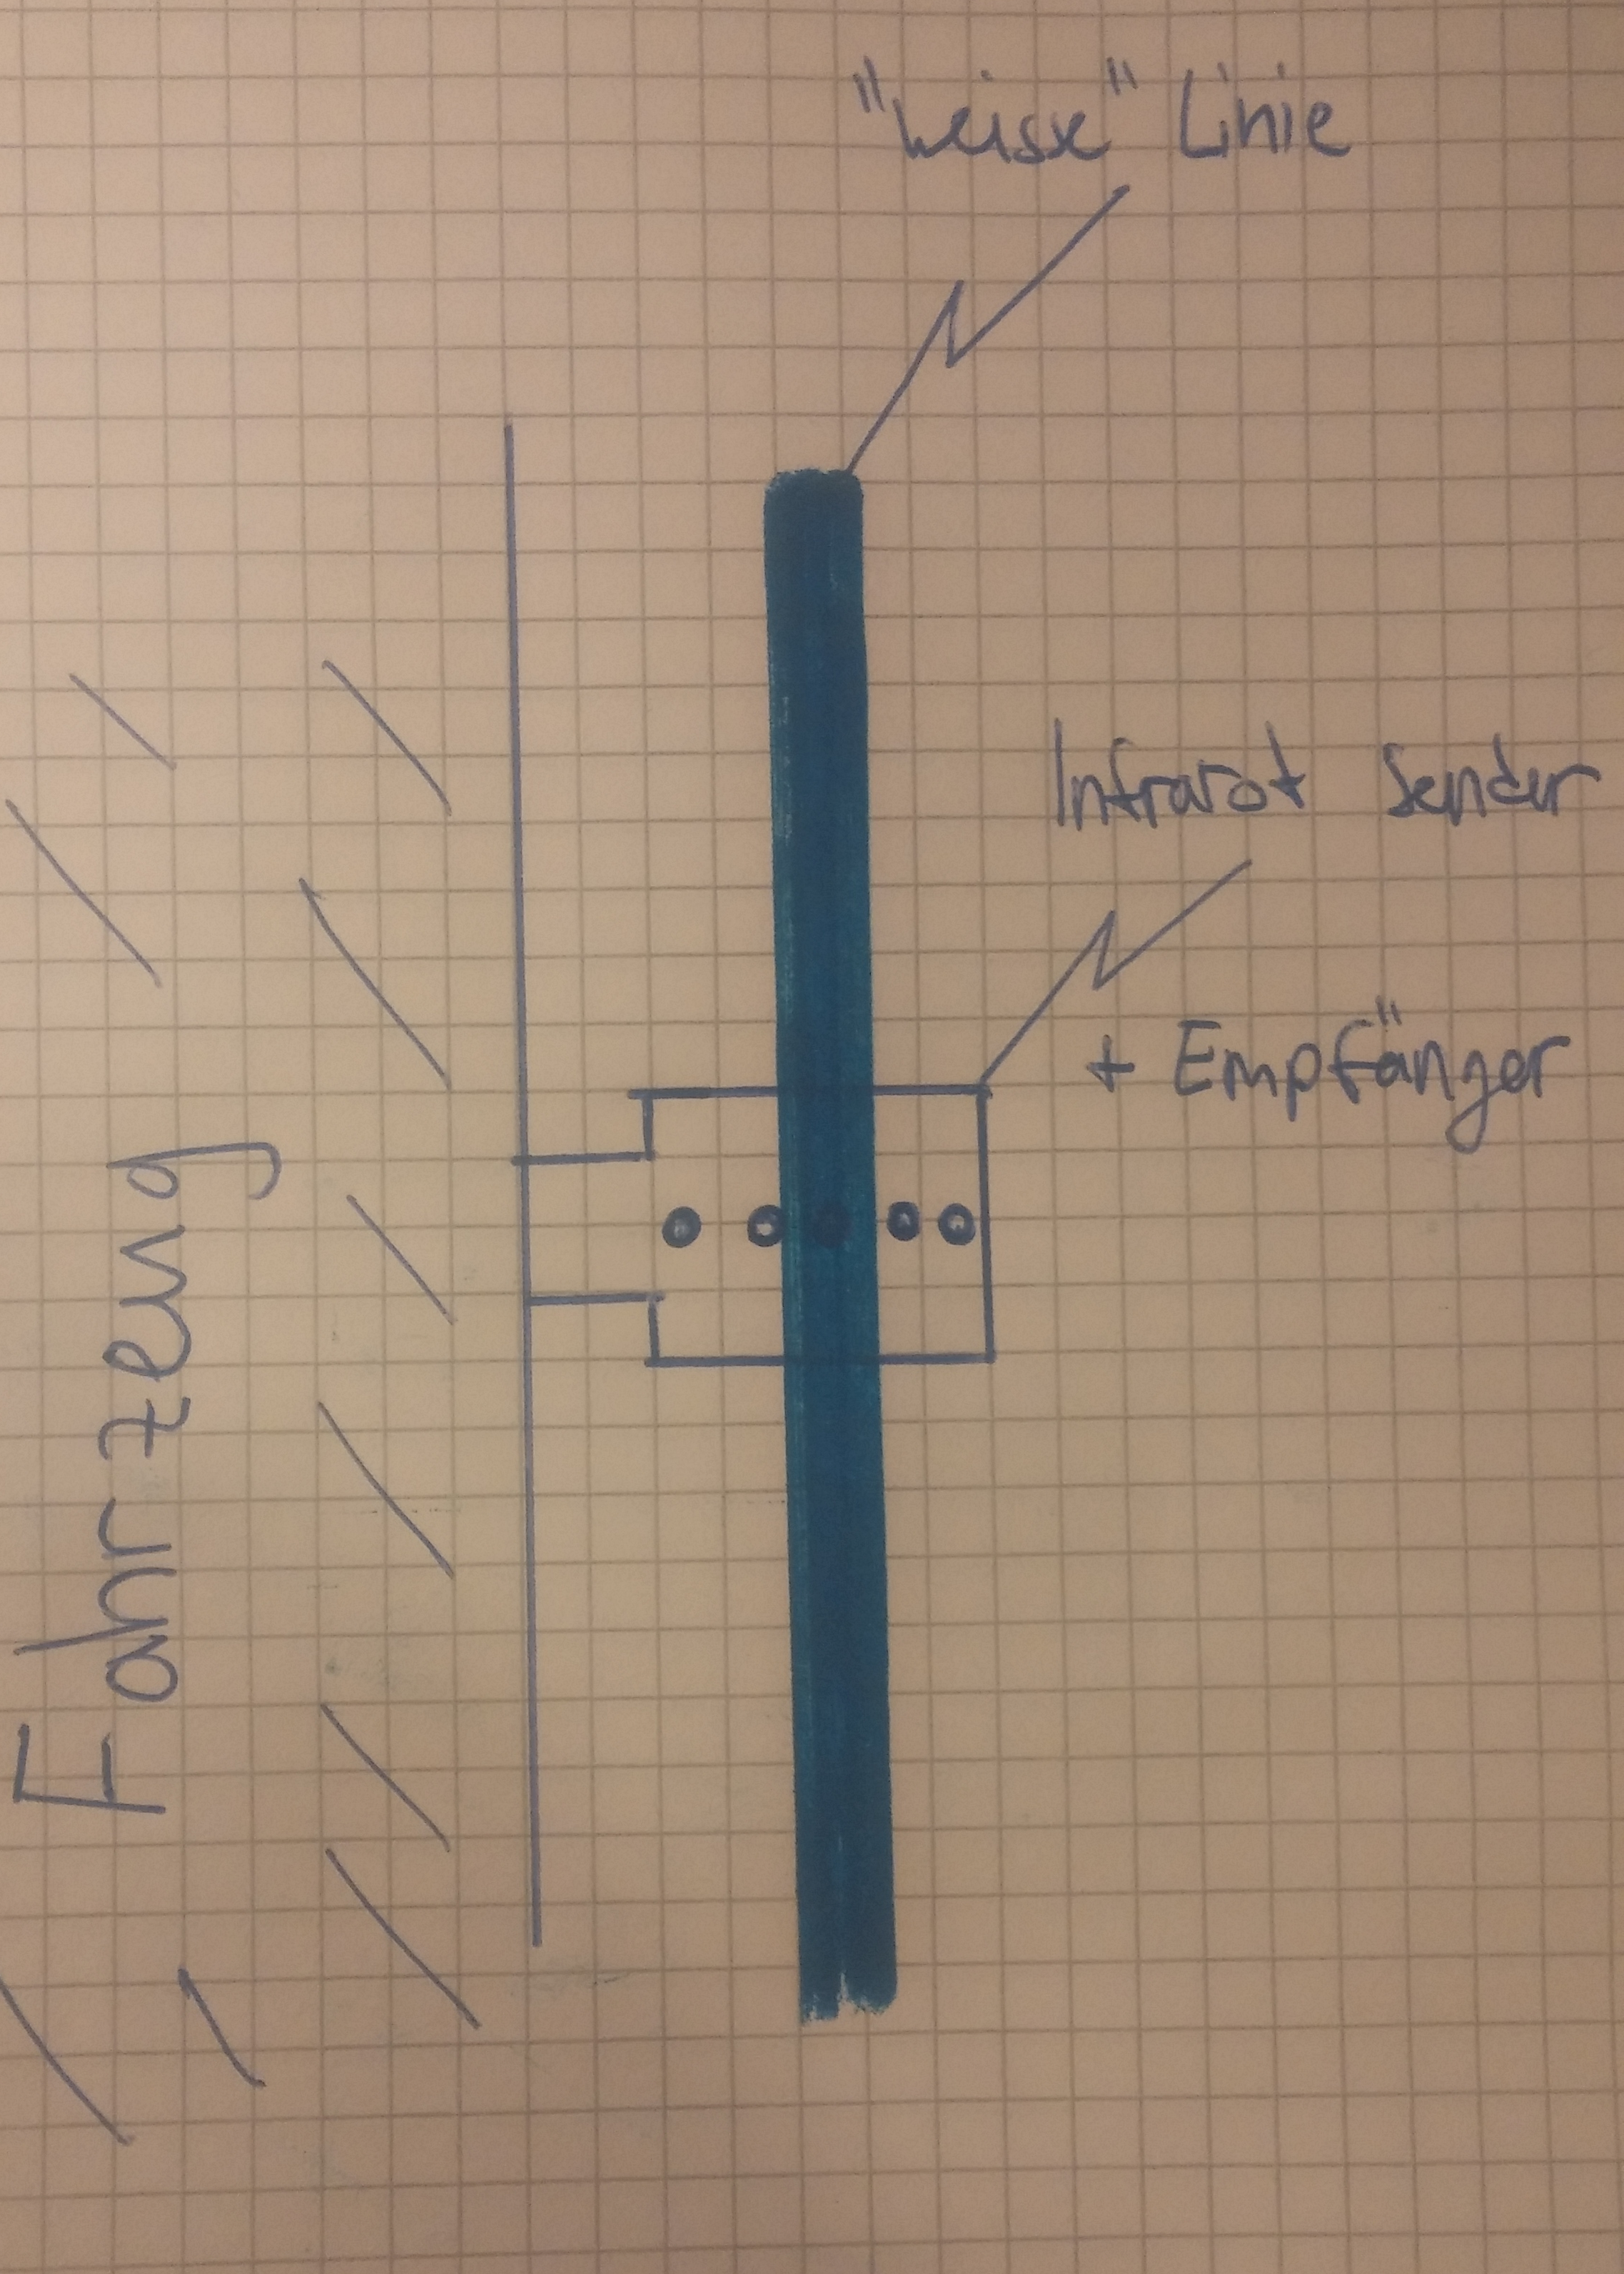
\includegraphics[width=\textwidth]{fig/Linienerkennung_1.png}
		\caption{1.Situation: Sensoren über der Linie}
	\end{subfigure}
	\hfill
	\begin{subfigure}[b]{0.36\textwidth}
		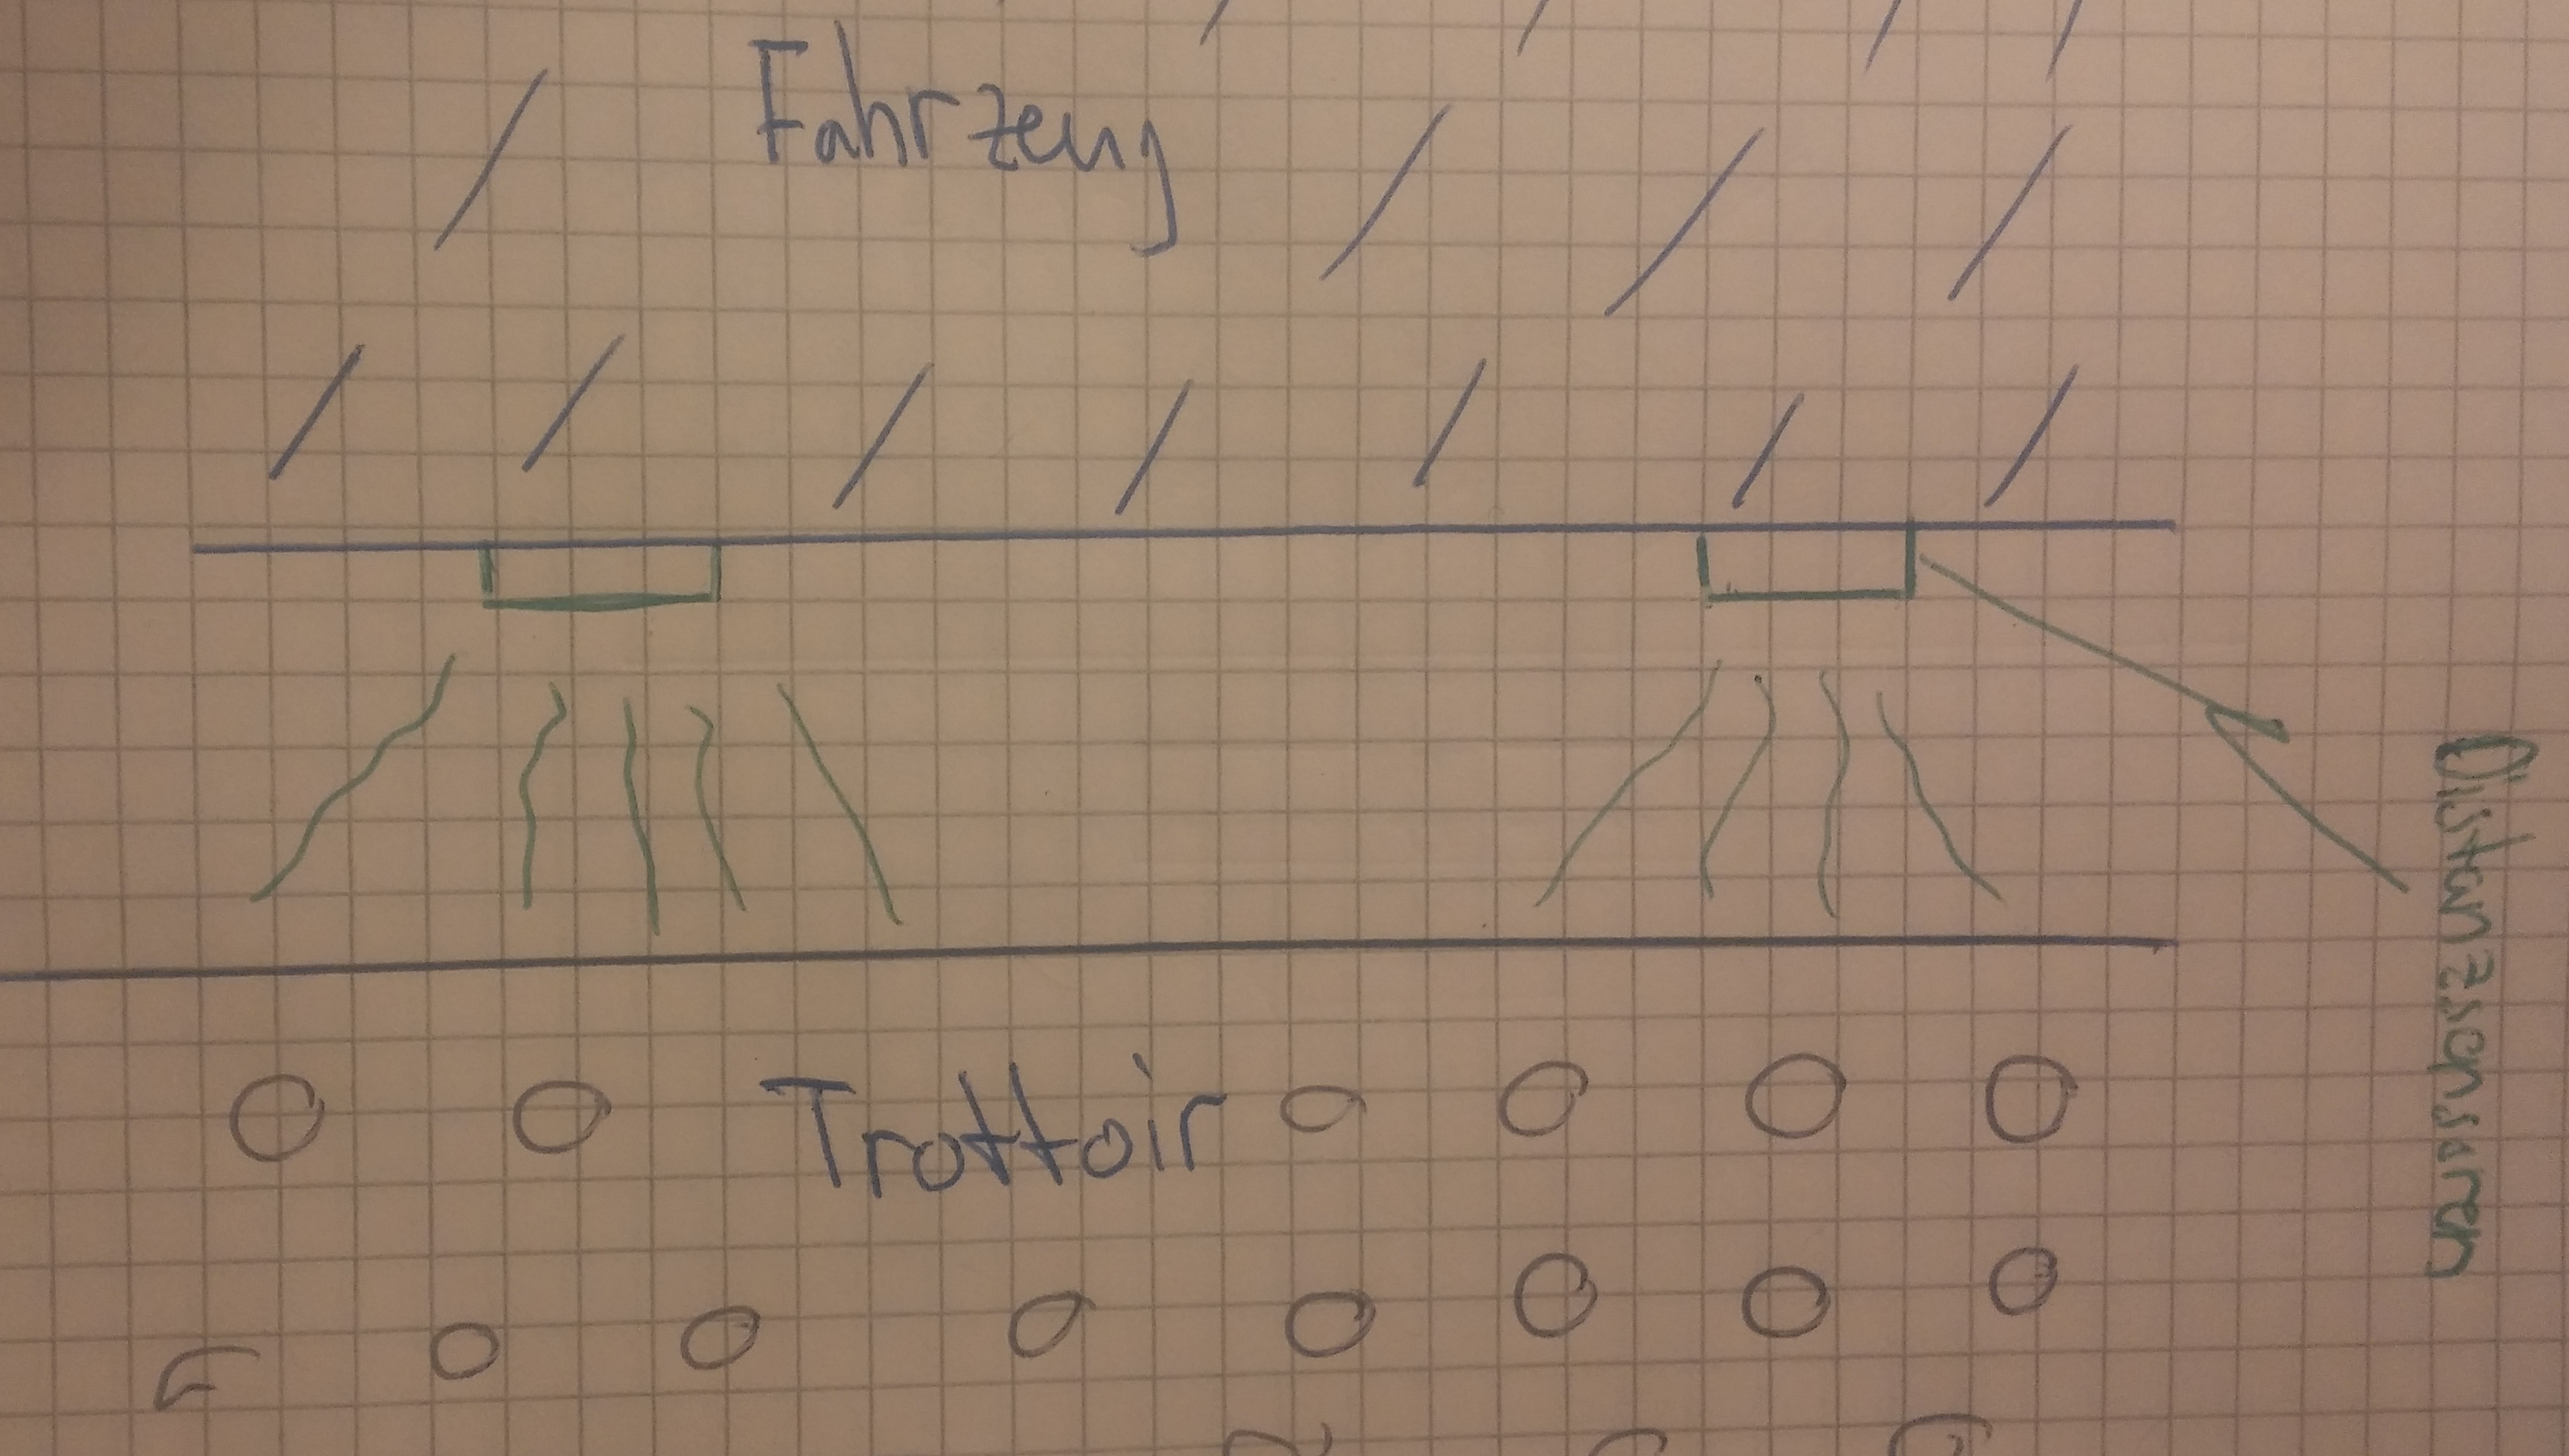
\includegraphics[width=\textwidth]{fig/Trottoirerkennung_1.png}
		\caption{2. Situation: Sensoren für die Abstandserkennung}
\end{subfigure}
	\caption{Mögliche Spurerkennung mit Distanzsensoren}\label{fig:animals}
\end{figure}



\begin{table}[h]
\begin{tabular}{p{0.5\textwidth} | p{0.5\textwidth}}


 \textbf{Vorteile} & \textbf{Nachteile} \\ \hline
	 
\begin{itemize}
\item Gut zu testen (Funktionsmuster)
\item Gute Präzision wird erwartet
\end{itemize}

 
 &
 
\begin{itemize}
\item Braucht externe Hardware und Verkabelung
\item Funktionsmuster zwingend notwendig
\end{itemize}

\end{tabular}
\end{table}

\begin{table}[h]
\begin{tabular}{p{0.5\textwidth}p{0.5\textwidth}}

 \textbf{Risiken} & \\ \hline
	 
\begin{itemize}
\item Die Linie lässt sich nicht Erkennen (ohne Konflikte mit der Anforderungsliste)
\item Das Trottoir ist zu wenig hoch damit es sich erkennen lässt
\end{itemize}
&
\begin{itemize}
\item Die Steuerung aufgrund der Linienerkennung ist nicht praktikabel
\end{itemize}

 
\end{tabular}
\end{table}

\pagebreak


%##############
\subsection{Bilderkennung}
Grafik

\begin{table}[h]
\begin{tabular}{p{0.5\textwidth} | p{0.5\textwidth}}


 \textbf{Vorteile} & \textbf{Nachteile} \\ \hline
	 
\begin{itemize}
\item Vorteil 1
\item Vorteil 2
\item Vorteil 3
\item ...
\end{itemize}

 
 &
 
\begin{itemize}
\item Nachteil 1
\item Nachteil 2
\item Nachteil 3
\item ...
\end{itemize}

\end{tabular}
\end{table}

\begin{table}[h]
\begin{tabular}{p{0.5\textwidth}p{0.5\textwidth}}


 \textbf{Risiken} & \\ \hline
	 
\begin{itemize}
\item Risiko 1
\item Risiko 2
\end{itemize}
&
\begin{itemize}
\item Risiko 3
\item ...
\end{itemize}

 
\end{tabular}
\end{table}

\pagebreak
% !TEX root = ../Dokumentation.tex
\subsection{Objekterkennung}

\subsubsection{Containererkennung}
Die Containererkennung hat das Ziel die richtigen Container zu erkennen und das genaue positionieren des Fahrzeuges zu ermöglichen. Dabei wird die Containererkennung wieder in zwei Teilaufgaben aufgeteilt. Die Containererkennung grob ist für die Erkennung der richtigen Farbe (und Form) zuständig. Die Containererkennung präzise ist für das Positionieren des Fahrzeuges notwendig. Diese zwei Fälle werden separat angeschaut.\\
\\
\textbf{Containererkennung präzise}\\
\\
\textbf{Funktionsbeschrieb}\\
Die präzise Containererkennung wird für das genaue Stoppen des Fahrzeuges gebraucht. Dieses Modul gibt den Trigger zum anhalten.\\
\\
\textbf{Komponentenbeschrieb}\\
Die Container Erkennung wird mit Hilfe von Distanzsensoren realisiert. Dafür sind Infrarot Distanzmesser oder Infrarot Reflexkoppler vorgesehen. Diese werden auf der rechten Seite des Fahrzeuges befestigt. Sobald ein Objekt in der Nähe ist ändert sich der Spannungswert, was einer Distanzänderung gleichkommt. 
\begin{figure} [hbp]
	\centering
	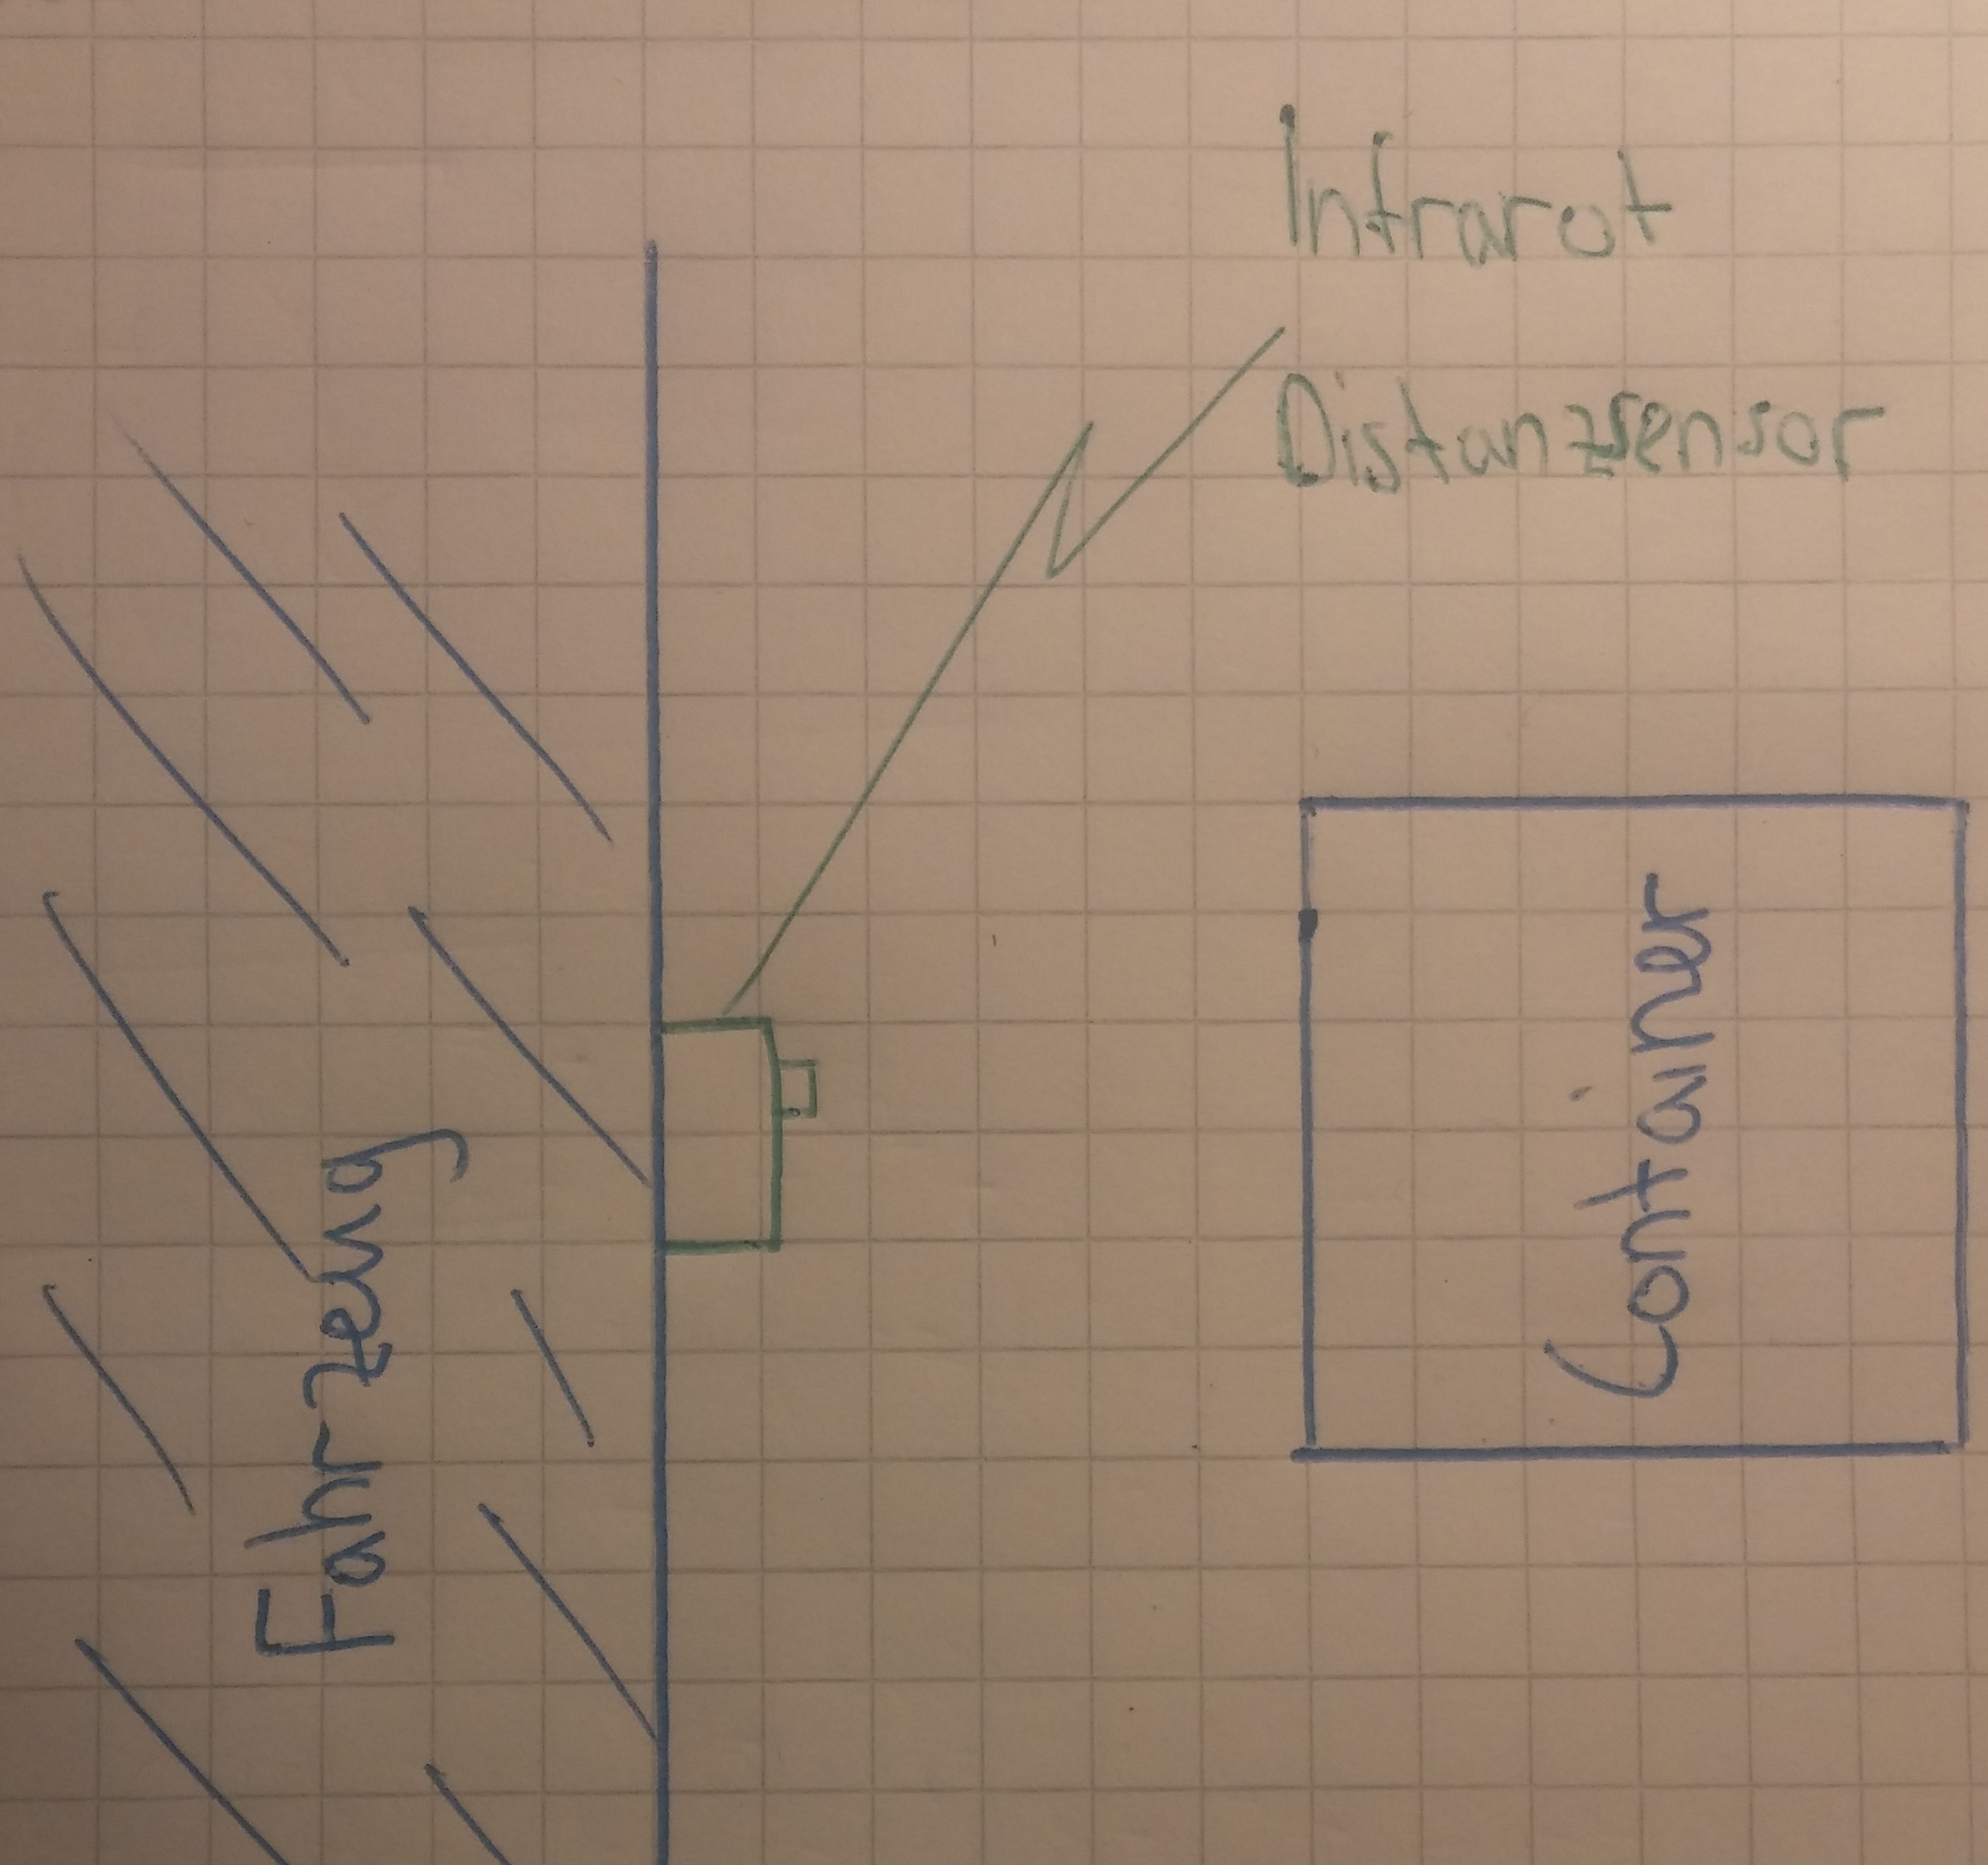
\includegraphics[width=0.35\textwidth]{./Images/InfrarotContainererkennung.png}
	\caption{Beispielhafte Containererkennung mit einem Infrarotsensor}
\end{figure}\\
\\
\textbf{Begründung}
\\
Die Positionierung mit einem Infrarotsensor ist die Ideale Lösung. Sie ist einfach zu realisieren im Vergleich zu einer Kamera oder einem Farbesensor und präziserer als ein Ultraschallsensor.\\
\\
\textbf{Testergebnisse}\\
Für die Ermittlung des besten Sensors wurde ein Ultraschall und Infrarotsensor als Funktionsmuster getestet. Der relativ grosse "Empfangswinkel", welcher der Ultraschallsensor aufweist, ist in dieser Anwendung nicht gewollt. Der Infrarotsensor ist diesbezüglich besser. Dieser ist jedoch Lichtempfindlich, jedoch sollte dieses Problem gelöst werden können.\
\\
\subsubsection{Rechtsvortritt}
\textbf{Funktionsbeschrieb}

\textbf{Komponentenbeschrieb}
\textbf{Begründung}
Wenn benötigt
\textbf{Berechnungen}
\textbf{Testergebnisse}

% !TEX root = Dokumentation.tex
\section{Projektmanagement}

\input{04_Projektmanagement/risikoanalyse.tex}
% !TEX root = Dokumentation.tex
\section{Schlussdiskussion}

% !TEX root = Dokumentation.tex
\subsection{Entwicklungskosten und -aufwand}
% !TEX root = Dokumentation.tex
\subsection{Lessons Learned}

Bei einer Projektarbeit mit interdisziplinärer Zusammenarbeit ist es wichtig sich früh auf einen Konsens zu einigen.
Für das Team war es wichtig sich immer gemeinsam zu entscheiden und so immer alle möglichen Auswirkungen im Blick zu haben.
Durch das Definieren von Schnittstellen bereits zu Begin, konnten viele Missverständnisse bereits in der Planungsphase bereinigt werden.

Gewisse OpenSource Lösungen bieten zwar eine breite und solide Palette von Funktionen an, sind aber schlecht auf eine spezifische Aufgabe skalierbar.
Ein begabteres Mitglied der Gruppe hat sich die Zeit genommen und mit vertieftem mathematischen Wissen einen sehr effizienten Algorithmus entwickelt.
Dieser schlanke, auf die Aufgabe zugeschnittene Algorithmus ermöglicht das Auswerten des Bildmaterials nahezu in Echtzeit.


Um eine Gruppe zu bilden und erfolgreich zu führen braucht es zwingend zwei Dinge.
Die gleichen Ziele und die gleichen Regeln für alle Mitglieder.
Doch wo es Regeln gibt, wird es auch Verstösse geben. Deshalb hat sich das Team früh auf eine adäquate Strafe geeinigt.
Kommt jemand zu spät oder gar nicht, so soll derjenige das nächste Mal Bier mitbringen.
So ist sichergestellt, dass genügend Motivation vorhanden ist und auch die anderen bei solch einem Missgeschick profitieren.
% !TEX root = Dokumentation.tex
\subsection{Offene Punkte}
% !TEX root = Dokumentation.tex
\subsection{Risiken}
% !TEX root = Dokumentation.tex
\subsection{Ausblick PREN2}

Ende PREN1 wurde ein Lösungskonzept ausgewählt und detailliert ausgearbeitet.
Die Aufgaben sind klar verteilt und das Team versteht sich gut. PREN2 geht nun nahtlos weiter und setzt die Planung in die Realität um.
Besonders ins Auge sticht die komplexe Navigation auf dem Spielfeld und das Zusammenspiel der vielen Sensoren.
Das Team freut sich auf die neuen Herausforderungen, die umso grösser sind, da ein Mitglied die Gruppe verlässt.


% !TEX root = Dokumentation.tex
\subsection{Fazit}

Ziel von PREN1 ist es ein Funktionskonzept zu einer Aufgabenstellung in Teamarbeit zu erstellen. Ende PREN1 hat die Gruppe nun ein plausibles und umsetzbares Konzept ausgearbeitet und ist selbst überzeugt davon. Es lässt sich sagen, dass die Projektplanung ein Erfolg ist. Besonders die variable Erkennung von Fahrbahn und Containern bereitete Sorgen. Deshalb wurde bereits in der Planung viel Zeit für die Problemlösung eingesetzt. Nun ist das Team zuversichtlich die Aufgabe korrekt und zeitig abzuschliessen und im Wettbewerb einen Platz in den vorderen Rängen zu belegen. Die Mitglieder arbeiten eingespielt und ecken nur selten an. So lässt sich das Projekt auch bezüglich Sozialkompetenz als erfolgreich bezeichnen. 






\end{document}